% -------------------------------------------------------------------------------- %

\begin{exercise}

Sei $H$ ein Hilbert-Raum mit Skalarprodukt $(\cdot; \cdot)_H$, $a: H \times H \to \R$ eine stetige, elliptische und symmetrische Bilinearform und $f \in H^\ast$ ein stetiges, lineares Funktional.
Weiter sei

\begin{align}
  J(v) := \frac{1}{2} a(v;v) - f(v),
  \quad
  v \in H.
\end{align}

\begin{enumerate}[label = \textbf{\alph*)}]

  \item Zeigen Sie, dass $u \in H$ genau dann eine Lösung von $a(u; \cdot) = f$ in $H$ ist, wenn es das Funktional $J$ auf $H$ minimiert.

  \item Sei nun $H_0 \subset H$ ein linearer Teilraum, $g \in H$ und $H_g := \Bbraces{v \in H: v - g \in H_0}$.
  Zeigen Sie, dass $u \in H_g$ genau dann eine Lösung von $a(u; \cdot) = f$ in $H_0$ ist, wenn es das Funktional $J$ auf $H_g$ minimiert.

\end{enumerate}

\end{exercise}

% -------------------------------------------------------------------------------- %

\begin{solution}

\phantom{}

\begin{enumerate}[label = \textbf{\alph*)}]

  \item Die Definitionen von \enquote{stetig} und \enquote{elliptisch} findet man in Exercise 7.

  \begin{align*}
    \Exists L > 0:
    \Forall u, v \in H:
    a(u; v) \leq L \norm[H]{u} \norm[H]{v},
    \quad
    \Exists M > 0:
    \Forall u, v \in H:
    a(u; u) \geq M \norm[H]{u}^2
  \end{align*}

  \begin{itemize}

    \item
    [\enquote{$\implies$:}]

    \begin{figure}[h!]
      \centering
      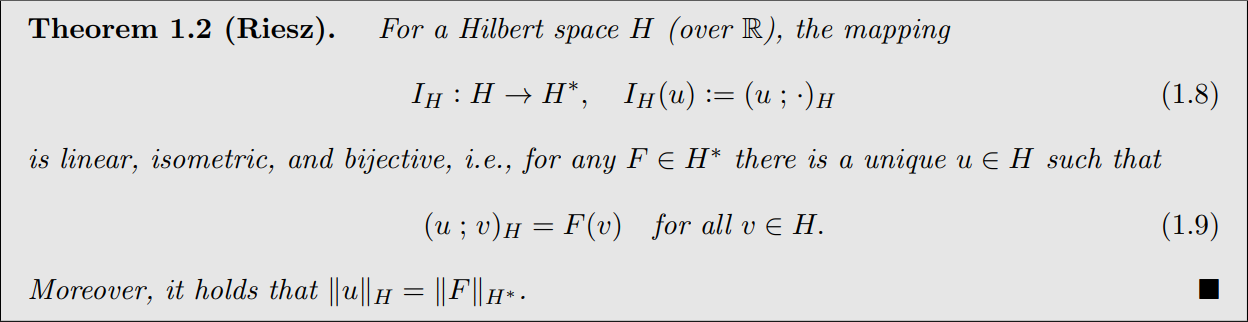
\includegraphics[width = 0.9 \textwidth]{../../../Fundament-LaTeX/images/NumPDEs/NumPDEs - Theorem 1.2 (Riesz).png}
    \end{figure}

    Die von $a$ induzierte Norm ist äquivalent zur Hilbertraumnorm.
    Wir erhalten daher mit Riesz eine eindeutige Lösung $u$ von $a(u; \cdot) = f$ in $H$, von der wir zeigen, dass sie das Funktional $J$ minimiert.
    Zunächst gilt $\Forall v \in H:$

    \begin{align*}
      2 (J(v) - J(u))
      & =
      a(v; v) - 2f(v) - a(u; u) + 2 f(u) \\
      & =
      a(v; v) -2a(u; v) + a(u; u) \\
      & =
      a(v-u; v) - a(u; v) + a(u; u) \\
      & =
      a(v-u; v) - a(v; u) + a(u; u) \\
      & =
      a(v-u; v) + a(u-v; u) \\
      & =
      a(v-u; v) - a(v-u; u) \\
      & =
      a(v-u; v-u) \\
      & \geq
      M \norm[H]{v-u}^2.
    \end{align*}

    \begin{align*}
      \implies
      J(v)
      \geq
      J(v) - \frac{1}{2} M \norm[H]{v-u}^2
      & \geq
      J(u)
    \end{align*}

    Also ist $u$ ein Minimum von $J$.

    \item
    [\enquote{$\impliedby$:}]
    Wir zeigen, dass Minima von $J$ ebenfalls eindeutig sind und somit jedes Minimum bereits mit der eindeutigen Lösung von $a(u;\cdot) = f$ übereinstimmen muss. \\

    Angenommen, $u \neq v$ seien Minima von $J$, dann folgt mit der oberen Rechnung

    \begin{align*}
      0 < M \norm[H]{v - u}^2 \leq 2(J(v) - J(u))
      \implies
      J(u) < J(v).
    \end{align*}

    Widerspruch!
    Minima von $J$ sind daher eindeutig.
    Damit ist bereits jedes (bzw. das) Minimum von $J$ auch eine (bzw. die) Lösung von $a(u; \cdot) = f$ in $H$.

  \end{itemize}

  \item Nach a) ist $u_0$ das Minimum von $J$ in $H_0$ genau dann, wenn es die eindeutige Lösung von $a(u; \cdot) = f$ auf $H_0$ ist.
  Wir wollen a) auf eine entsprechende Funktion $f_g$ anwenden.

  \begin{align*}
    f_g:
    H_0 \to \R:
    v_0 \mapsto f(v_0)  - a(g; v_0)
  \end{align*}

  \begin{align*}
    \stackrel{\text{a)}}{\implies}
    \Exists u_g \in H_0:
    \Forall v_0 \in H_0:
    a(u_g; v_0) = f_g(v_0)
  \end{align*}

  Damit folgt für $u := u_g + g$, dass

  \begin{align*}
    a(u; v_0)
    =
    a(u_g; v_0) + a(g; v_0) = f_g(v_0) + a(g; v_0)
    =
    f(v_0).
  \end{align*}

  Wir führen eine, zu der aus a),  analoge Abschätzung für $v_0 + g \in H_g = H_0 + g$ durch.

  \begin{align*}
    2(J(v_0 + g) - J(u_g + g))
    & =
    a(v_0 + g; v_0 + g) - a(u_g + g; u_g + g) + 2f(u_g - v_0) \\
    & =
    a(v_0; v_0) + a(g; g) + 2a(g; v_0) - a(u_g; u_g) - a(g; g) - 2a (g; u_g) + 2 f(u_g - v_0) \\
    & =
    a(v_0; v_0)  - a(u_g; u_g) + 2(f(u_g - v_0) - a(g; u_g - v_0)) \\
    & =
    a(v_0; v_0)  - a(u_g; u_g) + 2f_g(u_g - v_0) \\
    & =
    a(v_0; v_0)  - a(u_g; u_g) + 2a(u_g; u_g - v_0) \\
    & =
    a(v_0; v_0)  + a(u_g; u_g) - 2a(u_g; v_0) \\
    & =
    a(v_0 - u_g; v_0 - u_g) \\
    & \geq M \norm[H]{v_0 - u_g}^2
  \end{align*}

  Analog zu a) folgt, dass $u = u_g + g$ das eindeutige Minimum von $J$ auf $H_g$ ist.

\end{enumerate}

\end{solution}

% -------------------------------------------------------------------------------- %
